%%%%%%%%%%%%%%%%%%%%%%%%%%%%%%%%%%%%%%%%%
% baposter Portrait Poster
% LaTeX Template
% Version 1.0 (15/5/13)
%
% Created by:
% Brian Amberg (baposter@brian-amberg.de)
%
% This template has been downloaded from:
% http://www.LaTeXTemplates.com
%
% License:
% CC BY-NC-SA 3.0 (http://creativecommons.org/licenses/by-nc-sa/3.0/)
%
%%%%%%%%%%%%%%%%%%%%%%%%%%%%%%%%%%%%%%%%%

%----------------------------------------------------------------------------------------
%	PACKAGES AND OTHER DOCUMENT CONFIGURATIONS
%----------------------------------------------------------------------------------------

\documentclass[a0paper,portrait, fontscale=0.4]{baposter}

\usepackage[font=small,labelfont=bf]{caption} % Required for specifying captions to tables and figures
\usepackage{booktabs} % Horizontal rules in tables
\usepackage{relsize} % Used for making text smaller in some places
% Supports of Russian fonts
\usepackage[T1]{fontenc}
\usepackage[english,russian]{babel}
\usepackage[utf8]{inputenc}
\usepackage{type1ec}
% Math
\usepackage{amsmath,amsthm, amssymb, latexsym}

\graphicspath{{figures/}} % Directory in which figures are stored

\definecolor{bordercol}{RGB}{40,40,40} % Border color of content boxes
\definecolor{headercol1}{RGB}{186,215,230} % Background color for the header in the content boxes (left side)
\definecolor{headercol2}{RGB}{80,80,80} % Background color for the header in the content boxes (right side)
\definecolor{headerfontcol}{RGB}{0,0,0} % Text color for the header text in the content boxes
\definecolor{boxcolor}{RGB}{186,215,230} % Background color for the content in the content boxes

\begin{document}

\background{ % Set the background to an image (background.pdf)
\begin{tikzpicture}[remember picture,overlay]
\draw (current page.north west)+(-2em,2em) node[anchor=north west]
{\includegraphics[height=1.1\textheight]{background}};
\end{tikzpicture}
}

\begin{poster}{
grid=true,
borderColor=bordercol, % Border color of content boxes
headerColorOne=headercol1, % Background color for the header in the content boxes (left side)
headerColorTwo=headercol2, % Background color for the header in the content boxes (right side)
headerFontColor=headerfontcol, % Text color for the header text in the content boxes
boxColorOne=boxcolor, % Background color for the content in the content boxes
headershape=roundedright, % Specify the rounded corner in the content box headers
headerfont=\Large\sf\bf, % Font modifiers for the text in the content box headers
textborder=rectangle,
background=user,
headerborder=open, % Change to closed for a line under the content box headers
boxshade=plain
}
{}
%
%----------------------------------------------------------------------------------------
%	TITLE AND AUTHOR NAME
%----------------------------------------------------------------------------------------
%
{\sf\bf Проектирование детектора солнечных космических лучей} % Poster title
{\vspace{1em} John Smith, James Smith, Jane Smith\\ % Author names
{\smaller j.smith@uni.edu, j.smith2@uni.edu, j.smith3@uni.eduhttps://www.overleaf.com/project/5c52cf78a492f852be631a50}} % Author email addresses
{\includegraphics[scale=1]{logoNpm.pdf}} % University/lab logo

%----------------------------------------------------------------------------------------
%	INTRODUCTION
%----------------------------------------------------------------------------------------

\headerbox{Введение}{name=introduction,column=0,row=0}{

В связи с освоением космоса растет спрос на космические приборы, включая детекторы частиц. Целью настоящей работы является разработка концепции детектора солнечных космических лучей. Установка будет использоваться для измерения энергетических спектров протонов и электронов солнечного ветра. Кроме того, этот детектор может предсказывать солнечные вспышки протонов, обнаруживая солнечные вспышки электронов. Эта технология обеспечит радиационную безопасность для космонавтов и электроники.

$~$

Требования к детектору:
\begin{itemize}
    \item Высокое разрешение для протонов с энергией от 10 МэВ до 100 МэВ
    \item Высокое разрешение для электронов с энергией от 1 МэВ до 10 МэВ
    \item Оптимальные масса-габаритные характеристики
\end{itemize}

}

%----------------------------------------------------------------------------------------
%	MATERIALS AND METHODS
%----------------------------------------------------------------------------------------

\headerbox{Конструкция детектора}{name=methods,column=0,below=introduction}{

Детектор представляет собой цилиндр, собранный из нескольких сцинтилляционных дисков. Эти диски имеют толщину от толстых на входе до более широких на конце детектора. Такая геометрия позволяет точно измерять частицы с низкой энергией и использовать меньше электроники для измерения частиц с высокой энергией без значительного уменьшения разрешения.

Принцип регистрации частиц основан на физике прохождения излучения сквозь вещество. Частицы теряют энергию при прохождении сквозь детектор. Тип частицы и ее начальную кинетическую энергию можно восстановить по кривой потерь, которая показывает зависимость количества энергии, поглощенной веществом на единицу длины прохода, от общего прохода частицы.

}

%----------------------------------------------------------------------------------------
%	CONCLUSION
%----------------------------------------------------------------------------------------

\headerbox{Результаты}{name=conclusion,column=0,below=methods}{
\begin{itemize}
    \item Спроектирован детектор солнечных космических лучей
    \item Собран макет детектора
    \item Проверена зависимость работы MPPC от температуры
    \item Разработана методика анализа данных
\end{itemize}

}


%----------------------------------------------------------------------------------------
%	REFERENCES
%----------------------------------------------------------------------------------------

\headerbox{References}{name=references,column=0,below=conclusion}{

\smaller % Reduce the font size in this block
\renewcommand{\section}[2]{\vskip 0.05em} % Get rid of the default "References" section title
\nocite{*} % Insert publications even if they are not cited in the poster

\bibliographystyle{unsrt}
\bibliography{references} % Use sample.bib as the bibliography file
}

%----------------------------------------------------------------------------------------
%	ACKNOWLEDGEMENTS
%----------------------------------------------------------------------------------------

\headerbox{Благодарности}{name=acknowledgements,column=0,below=references, above=bottom}{

\smaller % Reduce the font size in this block
Работа сделана при поддержке гранта РНФ 17-72-20134.
} 
%----------------------------------------------------------------------------------------
%	RESULTS 1
%----------------------------------------------------------------------------------------

\headerbox{Методика измерения и анализ входных сигналов}{name=results1,span=2,column=1,row=0}{ % To reduce this block to 1 column width, remove 'span=2'

%------------------------------------------------

\begin{center}
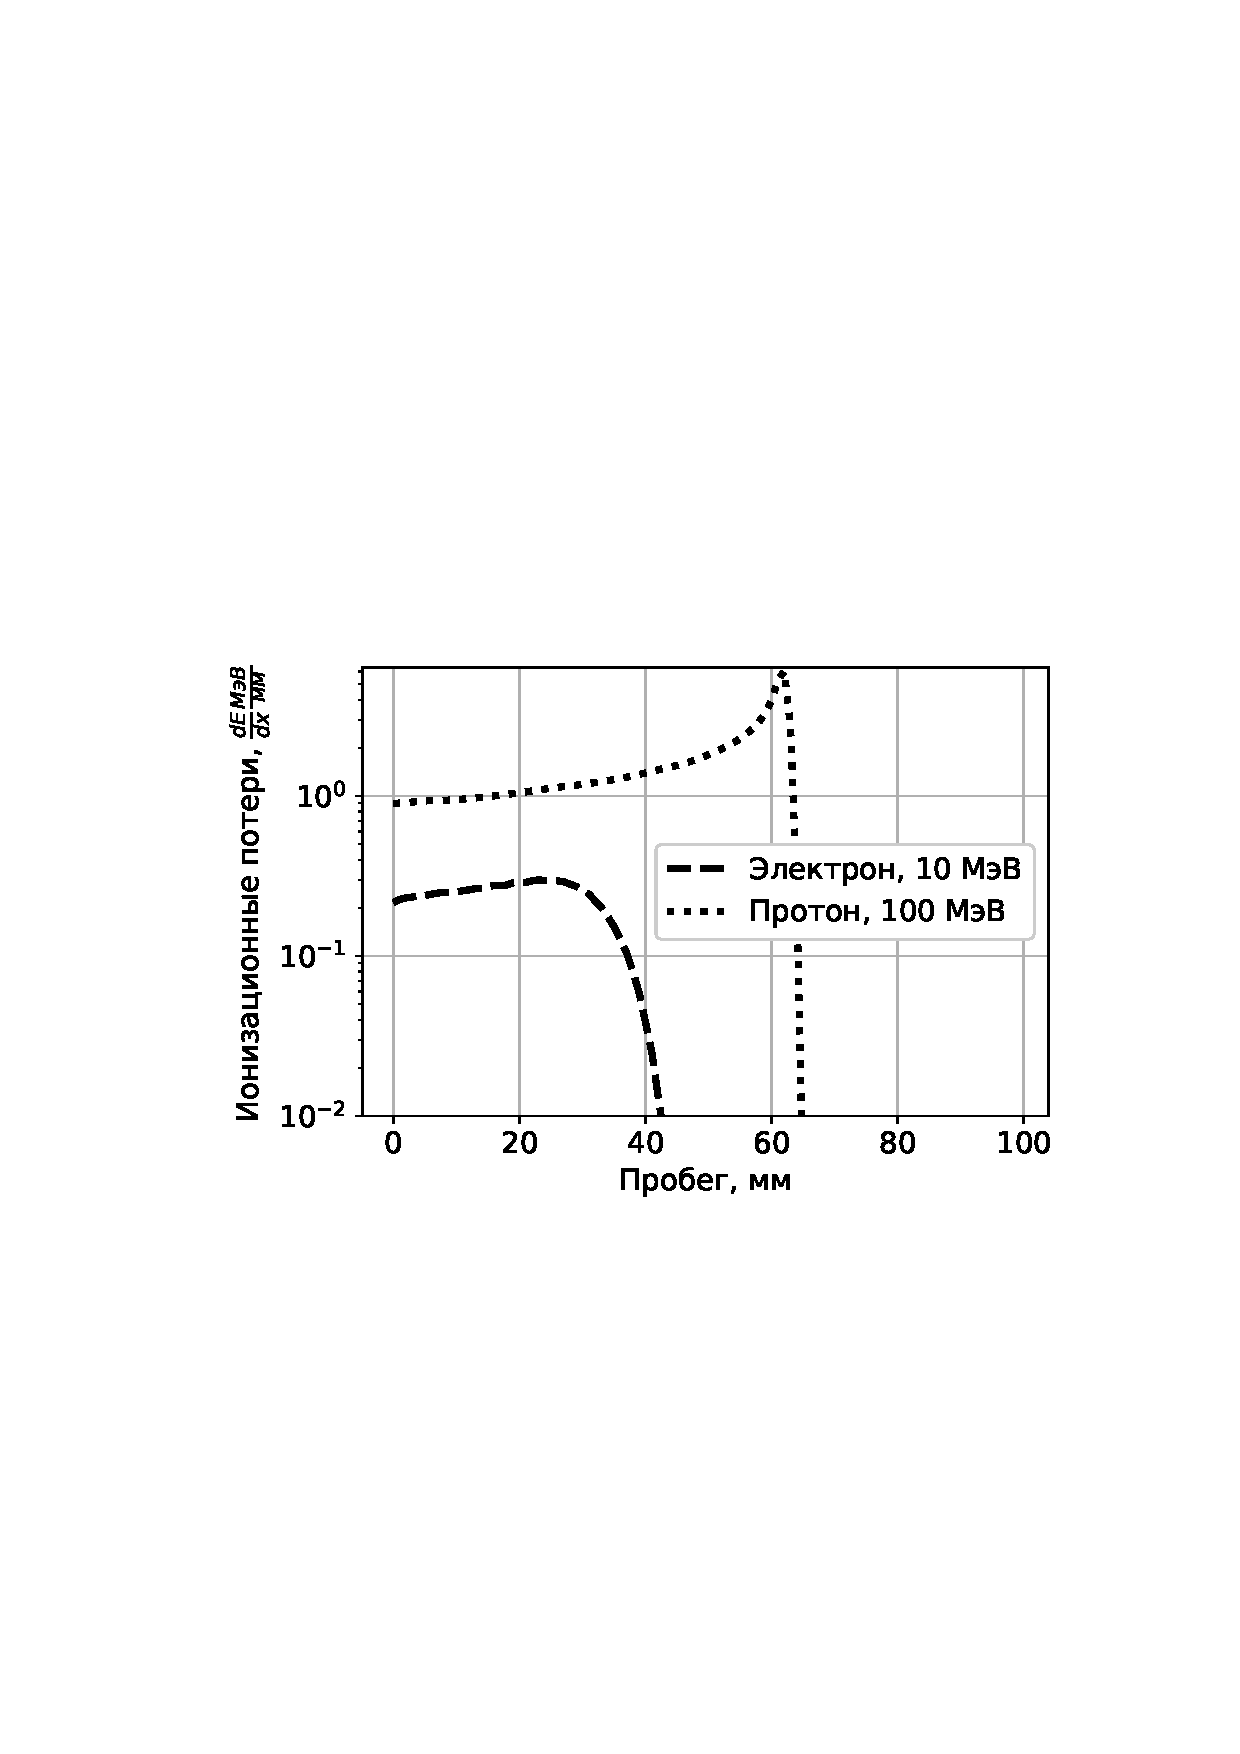
\includegraphics[width=0.1\linewidth]{01_bregg.pdf}

\captionof{figure}{Возможные способы крепления MPPC к шайбе детектора. \textcolor{green}{Перерисовать картикнки, сделать их одинковой высоты на прозрачном фоне}}
\end{center}

%------------------------------------------------

Существует два режима работы детектора: 

\begin{itemize}
    \item{Счётный. Включается, когда скорость счета электроники выше скорости прибытия частиц. В этом режиме частицы анализируются отдельно.} 
    \item{Интегральный. Скорость прихода частиц больше скорости счета электроники, например, во время солнечных вспышек.}
\end{itemize}
Интегральный режим можно анализировать несколькими способами: фитированием, регуляризацией Турчина и методом наименьших квадратов. Метод наименьших квадратов можно кратко описать следующим образом:

\begin{itemize}
    \item{Восстановленный спектр ищется в виде разложения по базису. В качестве базисных функций взяты полиномы Бернштейна:}
\end{itemize}
\begin{equation}
    \phi(E) = \sum T_n(E) \phi_n
\end{equation}
\begin{itemize}
    \item{Пусть функция потерь на j-ой шайбе детектора будет равна $K_j(E)$, где E - начальная кинетическая энергия частицы. На рисунке 7 показаны графики функции потерь. Полная потеря энергии в диске j может быть найдена следующим образом :}
\end{itemize}
\begin{equation}
    f_j = \int K_j(E) phi(E) d E
\end{equation}
\begin{itemize}
    \item{Cледовательно, $\phi_n$ может быть найдена путём решения следующей системы линейных уравнений:}
\end{itemize}
\begin{equation}
    f_j = \sum \phi_n \int K_j(E) T_n(E) d E = \sum \phi_n C_{j n}
\end{equation}
\begin{itemize}
    \item{Система переопределена, поэтому решение может быть найдено методом наименьших квадратов:}
\end{itemize}
\begin{equation}
    \phi = \left(C^TC\right)^{-1}C^T f
\end{equation}
%------------------------------------------------
}

%----------------------------------------------------------------------------------------
%	RESULTS 2
%----------------------------------------------------------------------------------------

\headerbox{Сборка и тестирование прототипа}{name=results2,span=1,column=1,below=results1,above=bottom}{ % To reduce this block to 1 column width, remove 'span=2'

Свет с сцинтиллятора регистрируется с помощью MPPC. В качестве фотодетекторов используются Hamamatsu SiPM S12575-015P. Закрепить на сцинтилляторе их можно двумя способами (рисунок 3): 
\begin{itemize}
    \item Прикрепить непосредственно к сцинтиллятору
    \item Снимать свет внутри шайбы оптоволокном и выводить его на MPPC
\end{itemize}

%------------------------------------------------

\begin{center}
\includegraphics[width=0.1\linewidth]{puck1.png}
\includegraphics[width=0.1\linewidth]{puck2.png}
\captionof{figure}{Возможные способы крепления MPPC к шайбе детектора. \textcolor{green}{Перерисовать картикнки, сделать их одинковой высоты на прозрачном фоне}}
\end{center}

%------------------------------------------------

У системы шайба + фотодетектор существует два существенных параметра: 
\begin{itemize}
    \item{Светосбор (определяет амплитуду сигнала на MPPC на единицу энергии, потерянной частицей в шайбе)}
    \item{Однородность светосбора (определяет, как сигнал зависит от точки входа частицы в шайбу)}
\end{itemize}
Эти параметры были измерены для двух возможных креплений MPPC. Оказалось, что светосбор в случае прямого контакта в 3 раза больше. Но конструкция с оптоволокном обладает практически полной однородностью светосбора. В связи с этим был выбран второй способ крепления MPPC.


Детектор рассчитан на работу при температурах от $-20~^\circ C$ до $+50~^\circ C$. При разных температурах MPPC требует подачи разного напряжения для оптимальной работы. В связи с этим на плату с MPPC установлена термопара. В документации SiPM приведена зависимость оптимального напряжения от температуры. В данной работе эта зависимость была проверена экспериментально.

Прототип детектора имеет следующую конструкцию (рисунок 5). Шайбы сцинтиллятора соединяются в цилиндр, который на ножках крепится на основную плату. К плате снизу присоединена электроника, на которой располагаются SiPM (рисунок 6). Из сцинтиллятора выведено оптоволокно, которое крепится непосредственно к MPPC.

\begin{center}
\includegraphics[width=0.49\linewidth]{detector.png}
\includegraphics[width=0.49\linewidth]{electronics.png}
\captionof{figure}{Слева: прототип детектора. Справа: электроника для считывания сигнала с детектора. \textcolor{green}{Обрезать лишние, унифицировать размер фото, сделать раздельные подписи}}
\end{center}
}

%----------------------------------------------------------------------------------------

\end{poster}

\end{document}